\documentclass{beamer}\usepackage[]{graphicx}\usepackage[]{xcolor}
% maxwidth is the original width if it is less than linewidth
% otherwise use linewidth (to make sure the graphics do not exceed the margin)
\makeatletter
\def\maxwidth{ %
  \ifdim\Gin@nat@width>\linewidth
    \linewidth
  \else
    \Gin@nat@width
  \fi
}
\makeatother

\definecolor{fgcolor}{rgb}{0.345, 0.345, 0.345}
\newcommand{\hlnum}[1]{\textcolor[rgb]{0.686,0.059,0.569}{#1}}%
\newcommand{\hlstr}[1]{\textcolor[rgb]{0.192,0.494,0.8}{#1}}%
\newcommand{\hlcom}[1]{\textcolor[rgb]{0.678,0.584,0.686}{\textit{#1}}}%
\newcommand{\hlopt}[1]{\textcolor[rgb]{0,0,0}{#1}}%
\newcommand{\hlstd}[1]{\textcolor[rgb]{0.345,0.345,0.345}{#1}}%
\newcommand{\hlkwa}[1]{\textcolor[rgb]{0.161,0.373,0.58}{\textbf{#1}}}%
\newcommand{\hlkwb}[1]{\textcolor[rgb]{0.69,0.353,0.396}{#1}}%
\newcommand{\hlkwc}[1]{\textcolor[rgb]{0.333,0.667,0.333}{#1}}%
\newcommand{\hlkwd}[1]{\textcolor[rgb]{0.737,0.353,0.396}{\textbf{#1}}}%
\let\hlipl\hlkwb

\usepackage{framed}
\makeatletter
\newenvironment{kframe}{%
 \def\at@end@of@kframe{}%
 \ifinner\ifhmode%
  \def\at@end@of@kframe{\end{minipage}}%
  \begin{minipage}{\columnwidth}%
 \fi\fi%
 \def\FrameCommand##1{\hskip\@totalleftmargin \hskip-\fboxsep
 \colorbox{shadecolor}{##1}\hskip-\fboxsep
     % There is no \\@totalrightmargin, so:
     \hskip-\linewidth \hskip-\@totalleftmargin \hskip\columnwidth}%
 \MakeFramed {\advance\hsize-\width
   \@totalleftmargin\z@ \linewidth\hsize
   \@setminipage}}%
 {\par\unskip\endMakeFramed%
 \at@end@of@kframe}
\makeatother

\definecolor{shadecolor}{rgb}{.97, .97, .97}
\definecolor{messagecolor}{rgb}{0, 0, 0}
\definecolor{warningcolor}{rgb}{1, 0, 1}
\definecolor{errorcolor}{rgb}{1, 0, 0}
\newenvironment{knitrout}{}{} % an empty environment to be redefined in TeX

\usepackage{alltt}
\usepackage{graphicx}
\usepackage{graphicx}
\usepackage{verbatim}
\usepackage{etoolbox}
\usepackage{everysel}
% \usepackage{enumitem}

%% This package allows text highlighting
\usepackage{soul}

%% This sets the theme of the presentation which controls
%% the formatting of the slides
\usetheme{Boadilla}

%% Turn off the navigation symbols
\setbeamertemplate{navigation symbols}{} 

%% Change the default itemize [ball]s to [circle]s
\setbeamertemplate{itemize items}[circle]

%% Change the default enumerate [ball]s to plain text
\setbeamertemplate{enumerate items}[default]

%% Load the enumitem package and ensure it works nicely with beamer
% \setitemize{label=\usebeamerfont*{itemize item}
%   \usebeamercolor[fg]{itemize item}
%   \usebeamertemplate{itemize item}}
% \setenumerate{label=\usebeamerfont*{enumerate item}
%   \usebeamercolor[fg]{enumerate item}
%   \usebeamertemplate{enumerate item}}

%% Set the author block so STATS 201/8 appears on every
\author{STATS 201/8}

%% Clear the date block
\date{}


\setbeamercolor{title}{bg=blue!40}
\setbeamerfont{title}{size=\LARGE,series=\bfseries}

%%Sectioning commands
\setbeamercolor{section title}{bg=blue!20}
\setbeamerfont{section title}{size=\large}

\setbeamertemplate{section page}{%
    \begingroup
        \begin{beamercolorbox}[sep=10pt,center,rounded=true,shadow=true]{section title}
        \usebeamerfont{section title}Section~\thechapter.\thesection \newline \insertsection\par
        \end{beamercolorbox}
		\vfill
    \endgroup
}

\newcommand{\BeginSection}[1]{\section{#1} \frame{\sectionpage}}
%\AtBeginSection[]{%
%    \begin{frame}
%        \sectionpage
%    \end{frame}
%}


%% This makes all equations blue
\AtBeginEnvironment{equation*}{\color{blue}}
\AtBeginEnvironment{align*}{\color{blue}}
\everymath{\color{blue}}

%% This puts a 0 point space between paragraphs, means we don't need to use vspace, or list environments if 
%% we don't want to
\setlength{\parskip}{0pt}


%% Russell: removes spaces after R input/output?
\setlength{\topsep}{0.5mm}

%% David: In addition to Russel's command to remove spaces after R input/output, these commands remove the space between R input/output.
%% Stackoverflow link: https://stackoverflow.com/questions/35734525/reduce-space-between-code-chunks-and-code-output-in-rmarkdown-beamer-presentatio
%% \setlength{\OuterFrameSep}{-2pt}
\makeatletter
\preto{\@verbatim}{\topsep=-1pt \partopsep=-1pt }
\makeatother

%% Some useful colors
\definecolor{darkgreen}{rgb}{0.176,0.486,0.031}
\definecolor{redbrown}{HTML}{950605}
\definecolor{darkred}{HTML}{d80605}


%% nice little macro for changing the font of R code
\newcommand{\rcode}[1]{\protect{\color{darkgreen}\texttt{#1}}}

%% macro for bold blue italics
\newcommand{\blueBoldEmph}[1]{{\color{blue}\textbf{\emph{#1}}}}

% ~iid macro
\newcommand{\iid }{\stackrel{iid}{\sim}}

%% Macro for t-test amd P-value
\newcommand{\ttest}{\emph{t}-test}
\newcommand{\pval}{\emph{P}-value}

%% Statistics operators 
\DeclareMathOperator{\Bias}{Bias}
\DeclareMathOperator{\Cov}{Cov}
\DeclareMathOperator*{\Cor}{Cor}
\DeclareMathOperator{\E}{E}
\DeclareMathOperator{\MSE}{MSE}
\DeclareMathOperator{\Odds}{Odds}
\DeclareMathOperator{\OR}{OR}
\DeclareMathOperator{\PMSE}{PMSE}
\DeclareMathOperator{\sd}{sd}
\DeclareMathOperator{\se}{se}
\DeclareMathOperator*{\Var}{Var}
\DeclareMathOperator{\logit}{logit}

%% Should see if can make this a mathop
\newcommand{\comb}[2]{\mbox{$\big(_{#2}^{#1}\big)$}}



\IfFileExists{upquote.sty}{\usepackage{upquote}}{}
\begin{document}
\newcommand{\thechapter}{5}



\title{Chapter 5: \\ Linear models with a 2-level categorical (factor) explanatory variable}
\institute{University of Auckland}

\begin{frame}
\titlepage
\end{frame}

\begin{frame}[t]
\frametitle{Learning Outcomes}
In this chapter you will learn about:
\begin{center}
\vspace{16pt}
\begin{minipage}{0.9\textwidth}
  \begin{itemize}
  \item Using a 2-level categorical variable as an explanatory variable in a linear model by using indicator variables
  \item Putting the two-sample \ttest{} into the linear model framework
  \item Relevant \rcode{R}-code.
  \end{itemize}
\end{minipage}
\end{center}
\end{frame}


%%%%%%%%%%%%%%%%%%%%%%%%%%%%%%%%%%%%%%%%%%%%%%%%%%%%%%%%%%%%%%%%%%%%%%%%%%%%%%%%%%%%%%%%%%%
\BeginSection{Using categorical variables as explanatory variables by using indicator variables}
%%%%%%%%%%%%%%%%%%%%%%%%%%%%%%%%%%%%%%%%%%%%%%%%%%%%%%%%%%%%%%%%%%%%%%%%%%%%%%%%%%%%%%%%%%%



\begin{frame}
\frametitle{New Example -- Exam marks vs Attendance}

We have gained some understanding about STATS 20x students' final exam marks and
how they are related to test and assignment scores, both of which are numeric explanatory variables.\\
\bigskip
Here, we are going to see if class attendance helps to explain exam score,
where class attendance (did or did not) is a categorical explanatory variable.\\
\bigskip
I am pretty sure we know there is going to be a relationship, but let us answer the question anyway.
This also lets us estimate the magnitude of the ``attendance effect''.
\end{frame}


\begin{frame}[fragile]
\frametitle{Exam marks vs Attendance}
\framesubtitle{The particular variables of interest}

\begin{tabular}{lp{15cm}}
\rcode{Exam} &  the student's Exam mark (out of 100) \\

\rcode{Attend} & whether the student regularly attended lectures or not

-- {\it Yes} or {\it No}.\footnote{This was measured by taking 4 rolls throughout the semester of  lecture  attendance. If a student was present for at least 3 of those 4 rolls, then they were recorded as a regular `attender'.}  \\

\end{tabular}

\bigskip

\textbf{Note:} As always, our question really is about the `typical' or average relationship. 
Some students may attend regularly but not do well in the exam, and vice-versa. 
That is part of the statistical variability, which we can deal with.
\end{frame}


\begin{frame}[fragile]
\frametitle{Exam marks vs Attendance\ldots}
\framesubtitle{Preliminary exploration of the data}
% note code get's rid of white space by pretending to submit but doing it on the sly later
\begin{knitrout}\scriptsize
\definecolor{shadecolor}{rgb}{0.969, 0.969, 0.969}\color{fgcolor}\begin{kframe}
\begin{alltt}
\hlstd{> }\hlcom{## Invoke the s20x library}
\hlstd{> }\hlkwd{library}\hlstd{(s20x)}
\hlstd{> }\hlcom{## Importing data into R}
\hlstd{> }\hlstd{Stats20x.df} \hlkwb{=} \hlkwd{read.table}\hlstd{(}\hlstr{"Data/STATS20x.txt"}\hlstd{,} \hlkwc{header}\hlstd{=T)}
\hlstd{> }\hlcom{## Change Attend from a character variable to a factor variable}
\hlstd{> }\hlstd{Stats20x.df}\hlopt{$}\hlstd{Attend} \hlkwb{=} \hlkwd{as.factor}\hlstd{(Stats20x.df}\hlopt{$}\hlstd{Attend)}
\hlstd{> }\hlcom{## Examine the data }
\hlstd{> }\hlstd{Stats20x.df}\hlopt{$}\hlstd{Attend[}\hlnum{1}\hlopt{:}\hlnum{20}\hlstd{]}
\end{alltt}
\begin{verbatim}
 [1] Yes Yes Yes Yes No  Yes Yes No  Yes Yes No  Yes No  No  No  Yes Yes No  Yes
[20] Yes
Levels: No Yes
\end{verbatim}
\end{kframe}
\end{knitrout}
The \rcode{Attend} variable has been formatted as a factor variable with two levels - \rcode{Levels: No Yes}.
\medskip

By default, \rcode{No} is the first level and \rcode{Yes} is the second level, because of alphabetical order -- but this can be changed if need be. 
In this case, we wish to contrast the attenders (\rcode{Yes}) against the non-attenders (\rcode{No})
and (as you will see later) this ordering of the levels suits us.
\end{frame}


\begin{frame}[fragile]
\frametitle{Exam marks vs Attendance\ldots}
\framesubtitle{Preliminary exploration of the data\ldots}

\begin{knitrout}\scriptsize
\definecolor{shadecolor}{rgb}{0.969, 0.969, 0.969}\color{fgcolor}\begin{kframe}
\begin{alltt}
\hlstd{> }\hlkwd{summaryStats}\hlstd{(Stats20x.df}\hlopt{$}\hlstd{Exam,Stats20x.df}\hlopt{$}\hlstd{Attend)}
\end{alltt}
\begin{verbatim}
    Sample Size     Mean Median  Std Dev Midspread
No           46 42.21739   40.5 16.34206     20.50
Yes         100 57.78000   58.0 17.67757     28.25
\end{verbatim}
\begin{alltt}
\hlstd{> }\hlkwd{plot}\hlstd{(Exam}\hlopt{~} \hlstd{Attend,} \hlkwc{data} \hlstd{= Stats20x.df,} \hlkwc{xlab}\hlstd{=}\hlstr{"Attendance"}\hlstd{)}
\end{alltt}
\end{kframe}
\end{knitrout}



\begin{figure}
  \centering
  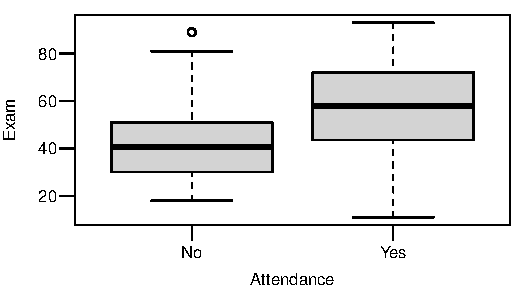
\includegraphics{figure/RC-H05-003}
\end{figure}
{\bf NOTE:} \rcode{Attend} is a factor, so \rcode{R} used a boxplot to display the data.
\end{frame}


\begin{frame}[fragile]
\frametitle{Exam marks vs Attendance\ldots}
\framesubtitle{Preliminary exploration of the data\ldots}

Here, we are asking how a student's attendance mark ($x$) is related to a their exam  ($y$) mark.\\
\bigskip 
As we are interested in the `typical' student, we want to see what the underlying trend is and how students vary (scatter) about that trend. \\
\bigskip 
Looking at the boxplot, it seems that regular attendance is associated with higher exam scores. 
Also, the equality of variance assumption seems okay. 
\bigskip

%We see that at least one non-attender earned a high exam score (relative to the other non-attenders), so we may have to keep an eye on this (e.g., there could be highly influential  points).
\end{frame}


\begin{frame}[fragile]
\frametitle{Exam marks vs Attendance\ldots}
\framesubtitle{Preliminary exploration of the data\ldots}

If you wish to use \rcode{trendscatter}, we need to create a new $x$ variable that is numerical.
We can do this by recoding non-attenders as $0$s and attenders as $1$s. \\
\bigskip
Here is the code for doing this recoding, with some checks to see that it has been successful.
\begin{knitrout}\scriptsize
\definecolor{shadecolor}{rgb}{0.969, 0.969, 0.969}\color{fgcolor}\begin{kframe}
\begin{alltt}
\hlstd{> }\hlcom{#Make a new variable Attend2 which is 1 if Attend = "Yes" and 0 otherwise}
\hlstd{> }
\hlstd{> }\hlcom{#Note how we use two equal signs, ==, to test equality}
\hlstd{> }\hlstd{Stats20x.df}\hlopt{$}\hlstd{Attend2} \hlkwb{=} \hlkwd{as.numeric}\hlstd{(Stats20x.df}\hlopt{$}\hlstd{Attend}\hlopt{==}\hlstr{"Yes"}\hlstd{)}
\hlstd{> }\hlkwd{with}\hlstd{(Stats20x.df,} \hlkwd{table}\hlstd{(Attend, Attend2))}
\end{alltt}
\begin{verbatim}
      Attend2
Attend   0   1
   No   46   0
   Yes   0 100
\end{verbatim}
\end{kframe}
\end{knitrout}
\bigskip
The \rcode{with} function lets us use the variables in the dataframe without having to type the dataframe name every time.
\end{frame}


\begin{frame}[fragile]
\frametitle{Exam marks vs Attendance\ldots}
\framesubtitle{Preliminary exploration of the data\ldots}
 \bigskip

\begin{knitrout}\scriptsize
\definecolor{shadecolor}{rgb}{0.969, 0.969, 0.969}\color{fgcolor}\begin{kframe}
\begin{alltt}
\hlstd{> }\hlkwd{trendscatter}\hlstd{(Exam}\hlopt{~} \hlstd{Attend2,} \hlkwc{data} \hlstd{= Stats20x.df)}
\end{alltt}
\end{kframe}
\end{knitrout}



\begin{figure}
  \centering
  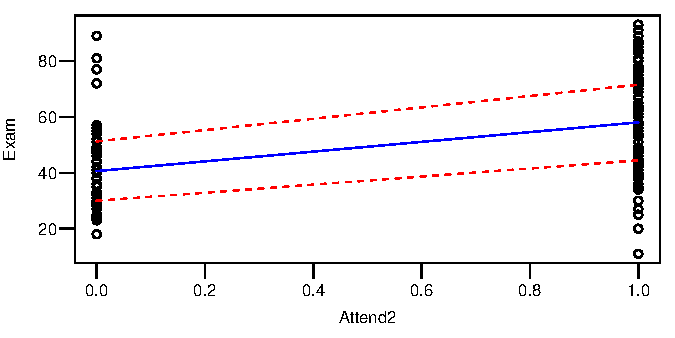
\includegraphics{figure/RC-H05-006}
\end{figure}

EOV assumption seems valid. 

\end{frame}


\begin{frame}[fragile]
\frametitle{Exam marks vs Attendance\ldots}
\framesubtitle{Fitting a linear model using \rcode{Attend2}}
Note that \rcode{Attend2} is a numeric explanatory variable (albeit with only two different values). So, we can fit a simple linear regression model to see how well \rcode{Attend2} explains \rcode{Exam}. What would this model tell us?
\medskip

The linear model for the expected value of \rcode{Exam} is
\[
\rcode{E[Exam|Attend2]}=\beta_0+\beta_1 \rcode{Attend2} \ .
\]
and so the full model equation is
\[
\rcode{Exam}_i=\beta_0+\beta_1 \rcode{Attend2}_i+\varepsilon_i \text{~where~} \varepsilon_i \iid N(0, \sigma^2) \ .
\]

If we use the notation \rcode{E[Exam|Attend2=0]} to denote the expected value of \rcode{Exam} when \rcode{Attend2}=0 then we have
\[
\rcode{E[Exam|Attend2=0]}=\beta_0 \ .
\]
Similarly, when \rcode{Attend2}=1
\[
\rcode{E[Exam|Attend2=1]}=\beta_0 + \beta_1\ .
\]


\end{frame}

\begin{frame}[fragile]
\frametitle{Exam marks vs Attendance\ldots}
\framesubtitle{Fitting a linear model using \rcode{Attend2}\ldots}
We see that $\beta_0$ is the mean exam mark for non-attenders and $\beta_0+\beta_1$ is the mean mark for attenders, and so $\beta_1$ is the difference in mean mark for attenders compared to non-attenders.
\bigskip

Our question of interest was to make inference about the "attendance effect" -- this "attendance effect" is simply $\beta_1$, so we can use the methods of inference about the slope of a linear model that we have already seen.
\bigskip

In particular, we know how to test the null hypothesis of no attendance effect, $H_0: \beta_1=0$, and how to obtain confidence intervals. Let's give it a go...


\end{frame}




\begin{frame}[fragile]
\frametitle{Exam marks vs Attendance\ldots}
\framesubtitle{Fitting a linear model using \rcode{Attend2}\ldots}

\medskip
\begin{knitrout}\scriptsize
\definecolor{shadecolor}{rgb}{0.969, 0.969, 0.969}\color{fgcolor}\begin{kframe}
\begin{alltt}
\hlstd{> }\hlstd{examattend2.fit} \hlkwb{=} \hlkwd{lm}\hlstd{(Exam}\hlopt{~} \hlstd{Attend2,} \hlkwc{data} \hlstd{= Stats20x.df)}
\hlstd{> }\hlkwd{summary}\hlstd{(examattend2.fit)}
\end{alltt}
\end{kframe}
\end{knitrout}

\begin{knitrout}\scriptsize
\definecolor{shadecolor}{rgb}{0.969, 0.969, 0.969}\color{fgcolor}\begin{kframe}
\begin{verbatim}
Coefficients:
            Estimate Std. Error t value Pr(>|t|)    
(Intercept)   42.217      2.547  16.578  < 2e-16 ***
Attend2       15.563      3.077   5.058 1.27e-06 ***
---
Residual standard error: 17.27 on 144 degrees of freedom
Multiple R-squared:  0.1508,	Adjusted R-squared:  0.145 
F-statistic: 25.58 on 1 and 144 DF,  p-value: 1.271e-06
\end{verbatim}
\end{kframe}
\end{knitrout}
Having to create the indicator variable\footnote{So-called because it indicates whether attendance is No or Yes. Some people call these dummy variables.} \rcode{Attend2} is a nuisance.
The good news is that the linear model function \rcode{lm} implicitly does this for us.
\medskip

Here we made the choice to recode non-attenders as $0$s and attenders as $1$s, rather than the other way around. This was deliberate -- it is the same choice that \rcode{lm} would make....see below.
\end{frame}



\begin{frame}[fragile]
\frametitle{Exam marks vs Attendance\ldots}
\framesubtitle{Fitting a linear model using \rcode{Attend}} 

We now fit a linear model to these data using the factor variable \rcode{Attend}.
The \rcode{lm} function automatically attributes \rcode{Attend=="No"} the zero value \footnote {This is called the \textbf{baseline} or reference level of the factor variable.} because \textbf{N}o comes before \textbf{Y}es in the alphabet, and \rcode{Attend=="Yes"} is attributed the value 1.

\begin{small}
\begin{knitrout}\scriptsize
\definecolor{shadecolor}{rgb}{0.969, 0.969, 0.969}\color{fgcolor}\begin{kframe}
\begin{alltt}
\hlstd{> }\hlstd{examattend.fit} \hlkwb{=} \hlkwd{lm}\hlstd{(Exam}\hlopt{~} \hlstd{Attend,} \hlkwc{data} \hlstd{= Stats20x.df)}
\hlstd{> }\hlkwd{summary}\hlstd{(examattend.fit)}
\end{alltt}
\end{kframe}
\end{knitrout}

\begin{knitrout}\scriptsize
\definecolor{shadecolor}{rgb}{0.969, 0.969, 0.969}\color{fgcolor}\begin{kframe}
\begin{verbatim}
Coefficients:
            Estimate Std. Error t value Pr(>|t|)    
(Intercept)   42.217      2.547  16.578  < 2e-16 ***
AttendYes     15.563      3.077   5.058 1.27e-06 ***
---
Residual standard error: 17.27 on 144 degrees of freedom
Multiple R-squared:  0.1508,	Adjusted R-squared:  0.145 
F-statistic: 25.58 on 1 and 144 DF,  p-value: 1.271e-06
\end{verbatim}
\end{kframe}
\end{knitrout}
\end{small}

What is the difference? Nothing really -- slightly different formats of the coefficient
names as \rcode{Attend2} is numerical and \rcode{Attend} is a categorical variable (factor).
\end{frame}


%%%%%%%%%%%%%%%%%%%%%%%%%%%%%%%%%%%%%%%%%%%%%%%%%%%%%%%%%%%%%%%%%%%%%%%%%%%%%%%%%%%%%%%%%%%
\BeginSection{Model checking and inference}
%%%%%%%%%%%%%%%%%%%%%%%%%%%%%%%%%%%%%%%%%%%%%%%%%%%%%%%%%%%%%%%%%%%%%%%%%%%%%%%%%%%%%%%%%%%


\begin{frame}[fragile]
\frametitle{Exam marks vs Attendance\ldots}
\framesubtitle{The fitted model}
Note that the p-value for \rcode{Attend} is very small, so we conclude that there is indeed a significant effect of attendance.
\medskip

The estimates of $\beta_0$ and $\beta_1$ are
\begin{knitrout}\scriptsize
\definecolor{shadecolor}{rgb}{0.969, 0.969, 0.969}\color{fgcolor}\begin{kframe}
\begin{verbatim}
(Intercept)   AttendYes 
   42.21739    15.56261 
\end{verbatim}
\end{kframe}
\end{knitrout}
That is, (formatted to 2 decimal places) $\hat{\beta}_0=42.22$ and $\hat{\beta}_1=15.56$.
\medskip

Using these estimated coefficients\footnote{Subject to verification of the model assumptions - stay tuned} 
our estimated values for the exam score of a `typical' student are:
\[
\widehat{\rcode{Exam}}= 42.22 + 15.56\times {\rcode{Attend2}}
\]
or
\[
\widehat{\rcode{Exam}}= 
\begin{cases}
  42.22 &\mbox{, for non-attenders and} \\
  42.22 + 15.56 &\mbox{, for attenders.}
\end{cases}
\]
\end{frame}


\begin{frame}[fragile]
\frametitle{Exam marks vs Attendance\ldots}
\framesubtitle{The fitted model\ldots}
Let's visualize the fit. Here we are plotting the `best' estimated straight line that we obtained from fitting our model using the indicator variable \rcode{Attend2}.

\begin{knitrout}\scriptsize
\definecolor{shadecolor}{rgb}{0.969, 0.969, 0.969}\color{fgcolor}\begin{kframe}
\begin{alltt}
\hlstd{> }\hlkwd{plot}\hlstd{(Exam} \hlopt{~} \hlstd{Attend2,} \hlkwc{data} \hlstd{= Stats20x.df)}
\hlstd{> }\hlcom{## Add the lm estimated line to this  plot  where a=intercept, b=slope}
\hlstd{> }\hlkwd{abline}\hlstd{(}\hlkwd{coef}\hlstd{(examattend.fit),}\hlkwc{lty}\hlstd{=}\hlnum{2}\hlstd{,} \hlkwc{col}\hlstd{=}\hlstr{"blue"}\hlstd{)}
\end{alltt}
\end{kframe}
\end{knitrout}



\begin{figure}
  \centering
  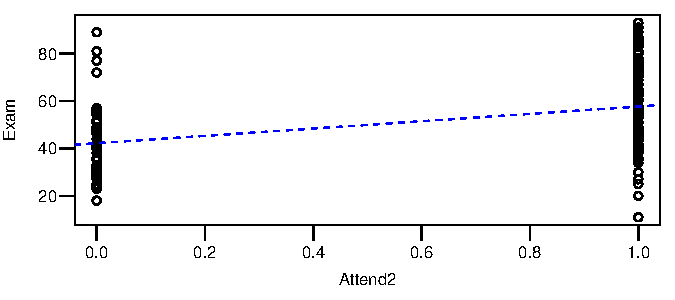
\includegraphics{figure/RC-H05-013}
\end{figure}

\end{frame}


\begin{frame}[fragile]
\frametitle{Exam marks vs Attendance\ldots}
\framesubtitle{The fitted model\ldots}

Here is the same thing using the factor variable \rcode{Attend}, with the fit overlaid on the boxplots.



\begin{figure}
  \centering
  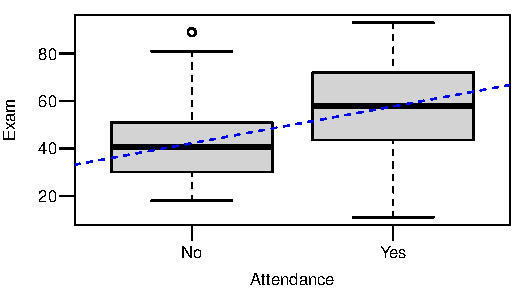
\includegraphics{figure/RC-H05-014}
\end{figure}

The two plots above essentially present the same information, 
repackaged in a slightly different way. 
\end{frame}


\begin{frame}[fragile]
\frametitle{Exam marks vs Attendance\ldots}
\framesubtitle{Checking assumptions}
We should check that our assumptions hold before we report (or use) the results from this analysis. Remember, we require independence, identical distribution and normality of the random components

\[
\varepsilon_i\iid N(0,\sigma^2).
\]

The assumptions (in order of importance):

\medskip
\textbf{i}id -- independence. We check this by investigating how we obtained the data.

\medskip
i\textbf{i}d -- identically distributed. This should result in the variation of the residuals being roughly constant (regardless of the fitted value) and the residuals more-or-less averaging around zero.  We can use \rcode{plot()} with the \rcode{which=1} argument.
\medskip

ii\textbf{d} -- Normality. We only check this having validated the first two assumptions, using \rcode{normcheck}.

\end{frame}

\begin{frame}[fragile]
\frametitle{Exam marks vs Attendance\ldots}
\framesubtitle{Checking our assumptions}

\begin{knitrout}\scriptsize
\definecolor{shadecolor}{rgb}{0.969, 0.969, 0.969}\color{fgcolor}\begin{kframe}
\begin{alltt}
\hlstd{> }\hlkwd{plot}\hlstd{(examattend.fit,}\hlkwc{which}\hlstd{=}\hlnum{1}\hlstd{)}
\end{alltt}
\end{kframe}
\end{knitrout}



\begin{figure}
  \centering
  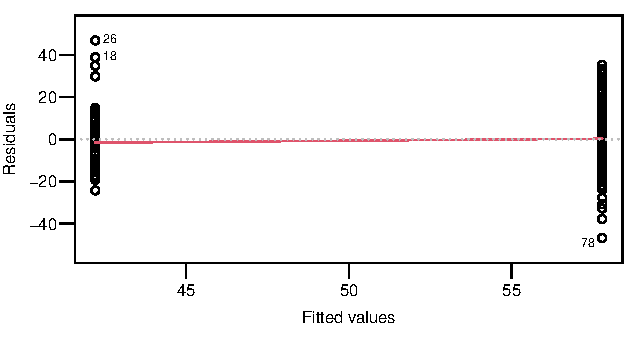
\includegraphics{figure/RC-H05-016}
\end{figure}
No cause for concern. 
\end{frame}


\begin{frame}[fragile]
\frametitle{Exam marks vs Attendance\ldots}
\framesubtitle{Checking our assumptions\ldots}
\medskip


\begin{knitrout}\scriptsize
\definecolor{shadecolor}{rgb}{0.969, 0.969, 0.969}\color{fgcolor}\begin{kframe}
\begin{alltt}
\hlstd{> }\hlkwd{normcheck}\hlstd{(examattend.fit)}
\end{alltt}
\end{kframe}
\end{knitrout}



\begin{figure}
  \centering
  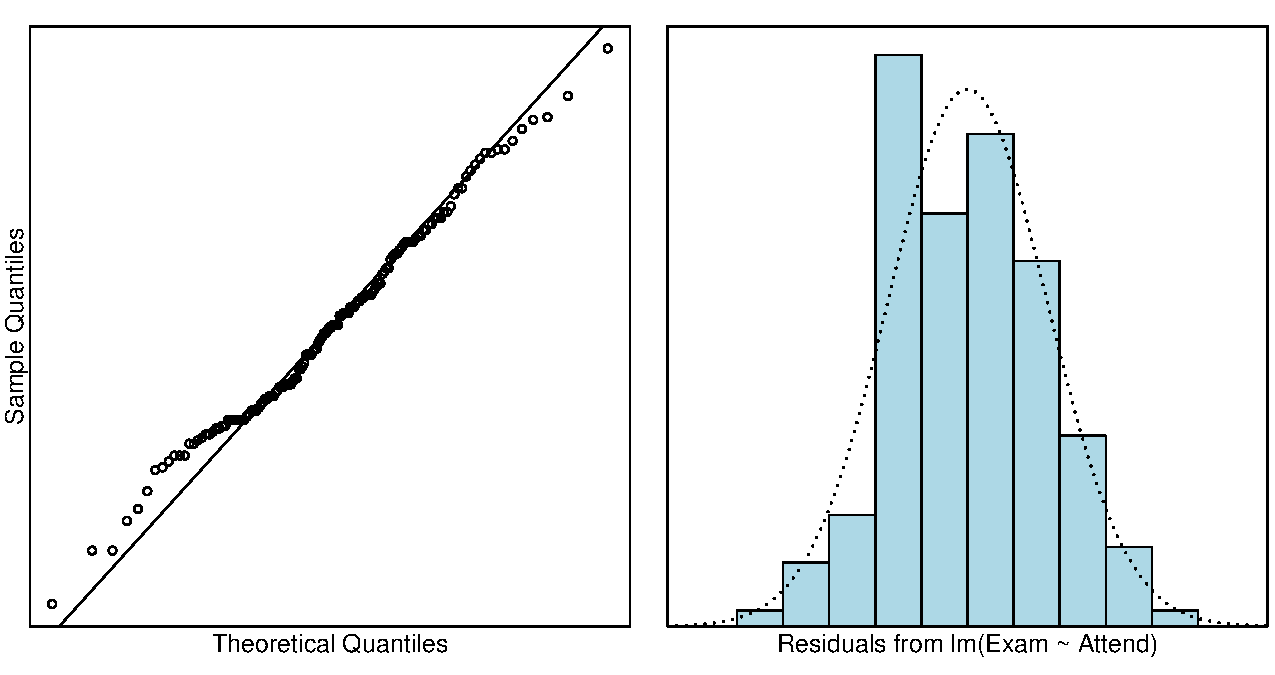
\includegraphics[scale=0.5]{figure/RC-H05-018}
\end{figure}

Looks good - the residuals appear to have a near normal distribution. 
\end{frame}


\begin{frame}[fragile]
\frametitle{Exam marks vs Attendance\ldots}
\framesubtitle{Checking our assumptions\ldots} \medskip

\begin{knitrout}\scriptsize
\definecolor{shadecolor}{rgb}{0.969, 0.969, 0.969}\color{fgcolor}\begin{kframe}
\begin{alltt}
\hlstd{> }\hlkwd{cooks20x}\hlstd{(examattend.fit)}
\end{alltt}
\end{kframe}
\end{knitrout}



\begin{figure}
  \centering
  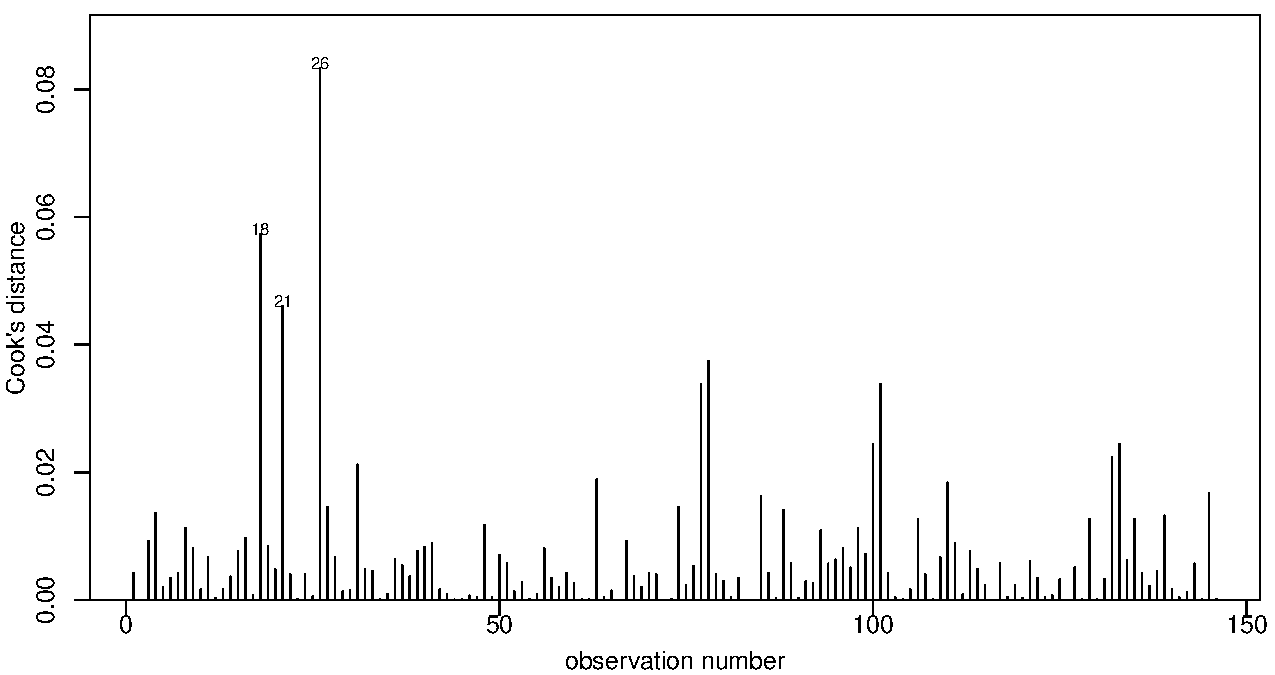
\includegraphics[scale=0.5]{figure/RC-H05-020}
\end{figure}

No unduly influential points.
\end{frame}


\begin{frame}[fragile]
\frametitle{Inference about Exam marks vs Attendance}
\framesubtitle{Testing the null hypothesis}
The model assumptions look to be reasonably well satisfied, so we can use the fitted model to make statistical inference (i.e., to answer questions of interest).
\bigskip

We begin by testing the null hypothesis that there is no effect of the explanatory variable \rcode{Attend}.\footnote{In this case, the null hypothesis corresponds to the \rcode{Exam} scores being iid.} Recall that this is $H_0:\beta_1=0$. 
\bigskip

\begin{knitrout}\scriptsize
\definecolor{shadecolor}{rgb}{0.969, 0.969, 0.969}\color{fgcolor}\begin{kframe}
\begin{alltt}
\hlstd{> }\hlkwd{coef}\hlstd{(}\hlkwd{summary}\hlstd{(examattend.fit))}
\end{alltt}
\begin{verbatim}
            Estimate Std. Error   t value     Pr(>|t|)
(Intercept) 42.21739   2.546517 16.578482 3.358318e-35
AttendYes   15.56261   3.076969  5.057773 1.271370e-06
\end{verbatim}
\end{kframe}
\end{knitrout}



The \pval{} for \rcode{AttendYes} is testing the null hypothesis $H_0: \beta_1=0$.
It is highly statistically significant $p=\ensuremath{1.27\times 10^{-6}}$, which is just over 1 in a million.
We have extremely strong evidence that attendance is related to exam score.

\end{frame}



\begin{frame}[fragile]
\frametitle{Inference about Exam marks vs Attendance\ldots}
\framesubtitle{Calculating confidence intervals for effect size}
We can get confidence intervals for $\beta_1$ (and $\beta_0$ if need be) by:
\begin{knitrout}\scriptsize
\definecolor{shadecolor}{rgb}{0.969, 0.969, 0.969}\color{fgcolor}\begin{kframe}
\begin{alltt}
\hlstd{> }\hlkwd{confint}\hlstd{(examattend.fit)}
\end{alltt}
\begin{verbatim}
                2.5 %   97.5 %
(Intercept) 37.184009 47.25077
AttendYes    9.480749 21.64447
\end{verbatim}
\end{kframe}
\end{knitrout}

\medskip
Here we can say that, on average,  regular attenders will obtain an increased exam mark of between  9.5 to 21.6 compared to non-attenders.

\medskip
Alternative wording would be: the expected exam mark of a student who regularly attends class is 9.5 to 21.6 marks higher than that of a non-attendee.

\end{frame}


\begin{frame}[fragile]
\frametitle{Inference about Exam marks vs Attendance\ldots}
\framesubtitle{Calculating confidence and prediction intervals}

We might also want to estimate and/or predict exam marks based on attendance status.

\medskip

Recall that we need to make a new dataframe containing the values of the explanatory
variable to be used for the prediction. In this case, that is just "No" and "Yes".

\begin{knitrout}\scriptsize
\definecolor{shadecolor}{rgb}{0.969, 0.969, 0.969}\color{fgcolor}\begin{kframe}
\begin{alltt}
\hlstd{> }\hlcom{## Create data frame of values of interest: Attend=="Yes" and "No"}
\hlstd{> }\hlcom{## Make sure that the names of vars are exactly the same as in the data frame}
\hlstd{> }\hlstd{preds.df} \hlkwb{=} \hlkwd{data.frame}\hlstd{(}\hlkwc{Attend} \hlstd{=} \hlkwd{c}\hlstd{(}\hlstr{"No"}\hlstd{,} \hlstr{"Yes"}\hlstd{))}
\hlstd{> }\hlkwd{predict}\hlstd{(examattend.fit, preds.df,} \hlkwc{interval} \hlstd{=} \hlstr{"confidence"}\hlstd{)}
\end{alltt}
\begin{verbatim}
       fit      lwr      upr
1 42.21739 37.18401 47.25077
2 57.78000 54.36619 61.19381
\end{verbatim}
\begin{alltt}
\hlstd{> }\hlkwd{predict}\hlstd{(examattend.fit, preds.df,} \hlkwc{interval} \hlstd{=} \hlstr{"prediction"}\hlstd{)}
\end{alltt}
\begin{verbatim}
       fit       lwr      upr
1 42.21739  7.710259 76.72452
2 57.78000 23.471673 92.08833
\end{verbatim}
\end{kframe}
\end{knitrout}
\end{frame}


\begin{frame}[fragile]
\frametitle{Inference about Exam marks vs Attendance\ldots}
\framesubtitle{Confidence and prediction intervals}

Here, we estimate the exam mark for non-regular attenders is between 37.2 and 47.3 on average, whereas for those who regularly attend it is between 54.4 and 61.2.

\medskip

For any individual student, if they are a non-regular attender then we predict their
exam mark to be between 7.7 and 76.7, or between 23.5 and 92.1 if they do attend regularly.

\medskip

The prediction intervals are very wide -- which is not surprising as regular attendance only explains 15\%  of the variation in exam score, and there is plenty of variability
between individual students.
\end{frame}


\begin{frame}[fragile]
\frametitle{Inference about Exam marks vs Attendance\ldots}
\framesubtitle{Confidence and prediction intervals}

Here is what the confidence (red)/prediction intervals (blue) look like:


\begin{figure}
  \centering
  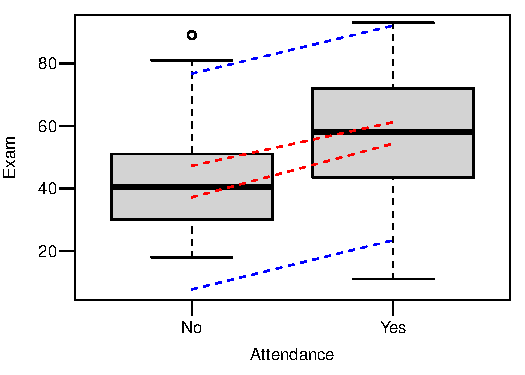
\includegraphics{figure/RC-H05-030}
\end{figure}

\end{frame}


%%%%%%%%%%%%%%%%%%%%%%%%%%%%%%%%%%%%%%%%%%%%%%%%%%%%%%%%%%%%%%%%%%%%%%%%%%%%%%%%%%%%%%%%%%%
\BeginSection{Putting the two-sample \ttest{} into the linear model framework}
%%%%%%%%%%%%%%%%%%%%%%%%%%%%%%%%%%%%%%%%%%%%%%%%%%%%%%%%%%%%%%%%%%%%%%%%%%%%%%%%%%%%%%%%%%%


\begin{frame}[fragile]
\frametitle{A recipe for subsequent analyses}
\frametitle{Two-sample \ttest{} in disguise}

We have just done an analysis to see if two groups (attendees and non-attendees) differ
in expected value.
You have encountered this scenario previously -- the two-sample \ttest{}.

\medskip

By default, the \rcode{t.test} function in \rcode{R} relaxes the equality of variance assumption,
so we have to explicitly tell it not to (using the \rcode{var.equal=TRUE} argument) 
if we want to reproduce our \rcode{lm} results exactly.

\begin{knitrout}\scriptsize
\definecolor{shadecolor}{rgb}{0.969, 0.969, 0.969}\color{fgcolor}\begin{kframe}
\begin{alltt}
\hlstd{> }\hlkwd{t.test}\hlstd{(Exam}\hlopt{~} \hlstd{Attend,} \hlkwc{var.equal}\hlstd{=}\hlnum{TRUE}\hlstd{,} \hlkwc{data} \hlstd{= Stats20x.df)}
\end{alltt}
\begin{verbatim}

	Two Sample t-test

data:  Exam by Attend
t = -5.0578, df = 144, p-value = 1.271e-06
alternative hypothesis: true difference in means between group No and group Yes is not equal to 0
95 percent confidence interval:
 -21.644468  -9.480749
sample estimates:
 mean in group No mean in group Yes 
         42.21739          57.78000 
\end{verbatim}
\end{kframe}
\end{knitrout}
\end{frame}


\begin{frame}[fragile]
\frametitle{Exam marks vs Attendance\ldots}
\framesubtitle{Two-sample \ttest{}}

The two-sample \ttest{} has a variant which relaxes the EOV assumption.
This is known as the \textbf{Welch} form of the \ttest{}, 
and is the default in the \rcode{t.test} function.  

\begin{knitrout}\scriptsize
\definecolor{shadecolor}{rgb}{0.969, 0.969, 0.969}\color{fgcolor}\begin{kframe}
\begin{alltt}
\hlstd{> }\hlkwd{t.test}\hlstd{(Exam}\hlopt{~} \hlstd{Attend,} \hlkwc{var.equal}\hlstd{=}\hlnum{FALSE}\hlstd{,} \hlkwc{data} \hlstd{= Stats20x.df)}
\end{alltt}
\end{kframe}
\end{knitrout}
or just
\begin{knitrout}\scriptsize
\definecolor{shadecolor}{rgb}{0.969, 0.969, 0.969}\color{fgcolor}\begin{kframe}
\begin{alltt}
\hlstd{> }\hlkwd{t.test}\hlstd{(Exam}\hlopt{~} \hlstd{Attend,} \hlkwc{data} \hlstd{= Stats20x.df)}
\end{alltt}
\begin{verbatim}

	Welch Two Sample t-test

data:  Exam by Attend
t = -5.2076, df = 94.09, p-value = 1.122e-06
alternative hypothesis: true difference in means between group No and group Yes is not equal to 0
95 percent confidence interval:
 -21.496121  -9.629096
sample estimates:
 mean in group No mean in group Yes 
         42.21739          57.78000 
\end{verbatim}
\end{kframe}
\end{knitrout}
\end{frame}


\begin{frame}[fragile]
\frametitle{Exam marks vs Attendance\ldots}
\framesubtitle{Two-sample \ttest{}\ldots}
The Welch form loses some degrees of freedom because it 
adds more uncertainty as we have to now estimate the variability of the sample in each group (attenders and non-attenders) rather than `pooling' them based on the EOV assumption. 

\bigskip

In this case, there is negligible difference between the standard and \textbf{Welch} forms of
the two-sample \ttest{}.

\end{frame}


\begin{frame}[fragile]
\frametitle{Summary}

We have now seen that \rcode{lm} can be used when the explanatory variable is numeric
(e.g., \rcode{Test} or \rcode{Assign}), 
and also when the explanatory variable is categorical (e.g., \rcode{Attend}).

\bigskip

When the explanatory variable is categorical, 
\rcode{lm} automatically creates numeric indicator variables to use in the model formula.
The indicator variables indicate the category level (relative to the baseline level) 
and take the value 0 or 1 -- for this reason they are sometimes referred to as indicator variables.

\bigskip
The natural question to ask here is: 
can we use \rcode{Test} and \rcode{Attend} {\em together} to explain exam score?

\bigskip
Stay tuned\ldots
\end{frame}




%%%%%%%%%%%%%%%%%%%%%%%%%%%%%%%%%%%%%%%%%%%%%%%%%%%%%%%%%%%%%%%%%%%%%%%%%%%%%%%%%%%%%%%%%%%
\BeginSection{\rcode{R} tips and relevant code}
%%%%%%%%%%%%%%%%%%%%%%%%%%%%%%%%%%%%%%%%%%%%%%%%%%%%%%%%%%%%%%%%%%%%%%%%%%%%%%%%%%%%%%%%%%%



\begin{frame}[fragile]
\frametitle{\rcode{R} tips and tricks}
\framesubtitle{Use of \rcode{-1} in model formulae}

In some situations it is useful to fit the model without a baseline level for the intercept.

\smallskip

This is easy, just add \rcode{-1} to the model formula.

\begin{knitrout}\scriptsize
\definecolor{shadecolor}{rgb}{0.969, 0.969, 0.969}\color{fgcolor}\begin{kframe}
\begin{alltt}
\hlstd{> }\hlstd{NoBaseline.fit}\hlkwb{=}\hlkwd{lm}\hlstd{(Exam}\hlopt{~} \hlstd{Attend}\hlopt{-}\hlnum{1}\hlstd{,} \hlkwc{data} \hlstd{= Stats20x.df)}
\hlstd{> }\hlkwd{summary}\hlstd{(NoBaseline.fit)}
\end{alltt}
\end{kframe}
\end{knitrout}

\begin{knitrout}\scriptsize
\definecolor{shadecolor}{rgb}{0.969, 0.969, 0.969}\color{fgcolor}\begin{kframe}
\begin{verbatim}
Coefficients:
          Estimate Std. Error t value Pr(>|t|)    
AttendNo    42.217      2.547   16.58   <2e-16 ***
AttendYes   57.780      1.727   33.45   <2e-16 ***
---
Residual standard error: 17.27 on 144 degrees of freedom
Multiple R-squared:  0.9064,	Adjusted R-squared:  0.9051 
F-statistic:   697 on 2 and 144 DF,  p-value: < 2.2e-16
\end{verbatim}
\begin{alltt}
\hlstd{> }\hlkwd{confint}\hlstd{(NoBaseline.fit)}
\end{alltt}
\begin{verbatim}
             2.5 %   97.5 %
AttendNo  37.18401 47.25077
AttendYes 54.36619 61.19381
\end{verbatim}
\end{kframe}
\end{knitrout}
Note: $R^2$ has no meaning when there is no intercept term in the model.
\end{frame}




\begin{frame}[fragile]
\frametitle{Most of the \rcode{R}-code you need for this chapter}

You do not need to create indicator variables as \rcode{R} does this for you. It will choose the baseline for you, so be careful.  You can change this if needed -- you will see an example of this soon. 
\medskip

\begin{knitrout}\scriptsize
\definecolor{shadecolor}{rgb}{0.969, 0.969, 0.969}\color{fgcolor}\begin{kframe}
\begin{alltt}
\hlstd{> }\hlstd{examattend.fit} \hlkwb{=} \hlkwd{lm}\hlstd{(Exam}\hlopt{~} \hlstd{Attend,} \hlkwc{data} \hlstd{= Stats20x.df)}
\end{alltt}
\end{kframe}
\end{knitrout}

This is equivalent to 
\begin{knitrout}\scriptsize
\definecolor{shadecolor}{rgb}{0.969, 0.969, 0.969}\color{fgcolor}\begin{kframe}
\begin{alltt}
\hlstd{> }\hlkwd{t.test}\hlstd{(Exam}\hlopt{~} \hlstd{Attend,} \hlkwc{var.equal}\hlstd{=}\hlnum{TRUE}\hlstd{,} \hlkwc{data} \hlstd{= Stats20x.df)}
\end{alltt}
\end{kframe}
\end{knitrout}
\bigskip

If it is clear that the two groups have massively different variances then one approach would be to abandon the use of a linear model and use the modified t-test without the equality of variance assumption\footnote{The modified t-test approach will {\bf never} be used in this class.}  
\begin{knitrout}\scriptsize
\definecolor{shadecolor}{rgb}{0.969, 0.969, 0.969}\color{fgcolor}\begin{kframe}
\begin{alltt}
\hlstd{> }\hlkwd{t.test}\hlstd{(Exam}\hlopt{~} \hlstd{Attend,} \hlkwc{var.equal}\hlstd{=}\hlnum{FALSE}\hlstd{,} \hlkwc{data} \hlstd{= Stats20x.df)}
\end{alltt}
\end{kframe}
\end{knitrout}
\medskip

{\bf However}, in most cases the technique shown in the next Chapter is a better way to cope with inequality of variance.


\end{frame}


\end{document}




